\documentclass[12pt,a4paper]{article}
\usepackage{pgfplots}
\usepackage{tikz}
\usepackage{import}
\usepackage[font=scriptsize,labelfont=bf]{caption}

\begin{document}

\newcommand*{\figuretitle}[1]{%
    {\centering%   <--------  will only affect the title because of the grouping (by the
    \textbf{#1}%              braces before \centering and behind \medskip). If you remove
    \par\medskip}%            these braces the whole body of a {figure} env will be centered.
}

\begin{figure}
\figuretitle{Simulations with duplication and loss}
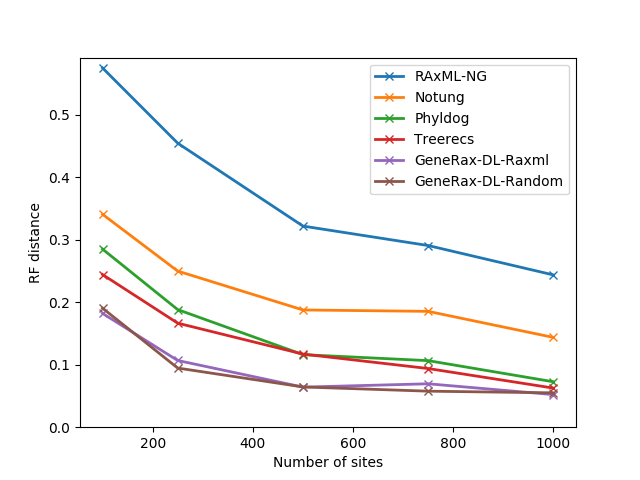
\includegraphics[scale=0.5]{sites.png}
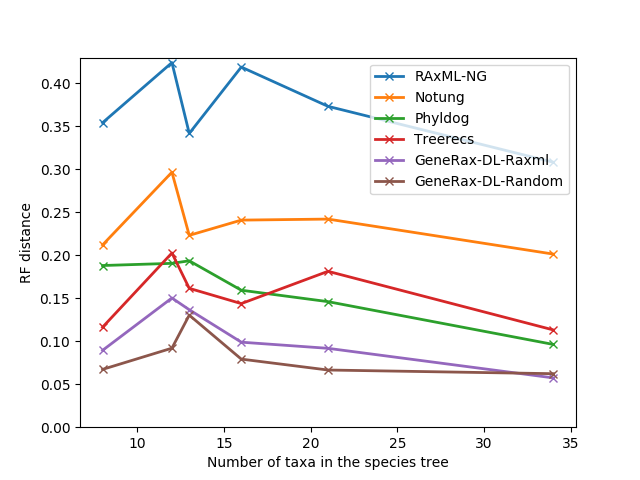
\includegraphics[scale=0.5]{species.png}
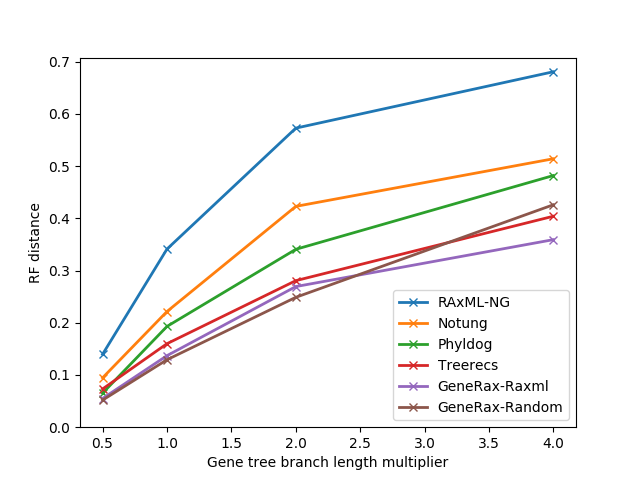
\includegraphics[scale=0.5]{bl.png}
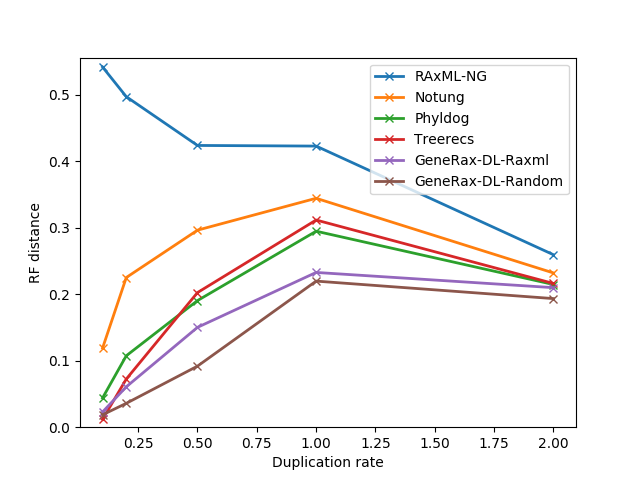
\includegraphics[scale=0.5]{rates.png}
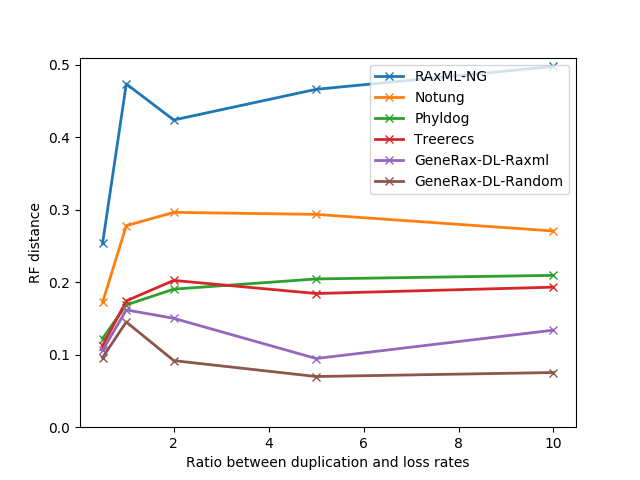
\includegraphics[scale=0.5]{dl_ratio.png}
\caption{On each plot, one parameter varies while the other ones are fixed. Notung, Phyldog, Treerecs and GeneRax-Raxml start from the RAxML-NG tree. RAxML-NG was ran from $10$ starting random trees. GeneRax-Random starts from a random tree. Notung and Treerecs need support values: we generated them with RAxML-NG and $100$ bootstrap trees.}
\end{figure}

\begin{figure}
\figuretitle{Simulations with duplication, transfer and loss}
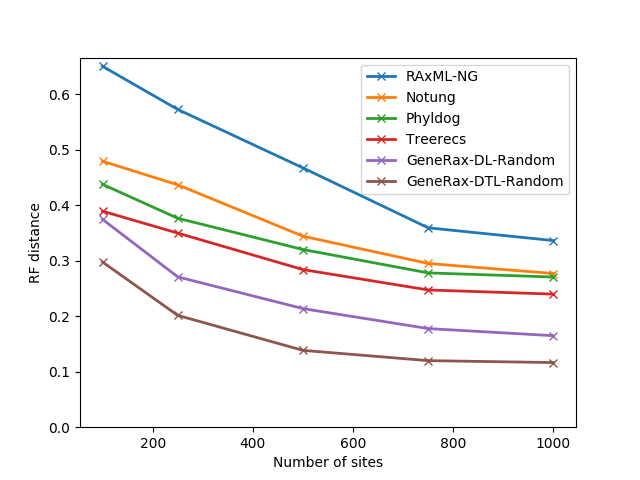
\includegraphics[scale=0.5]{sites_dtl.png}
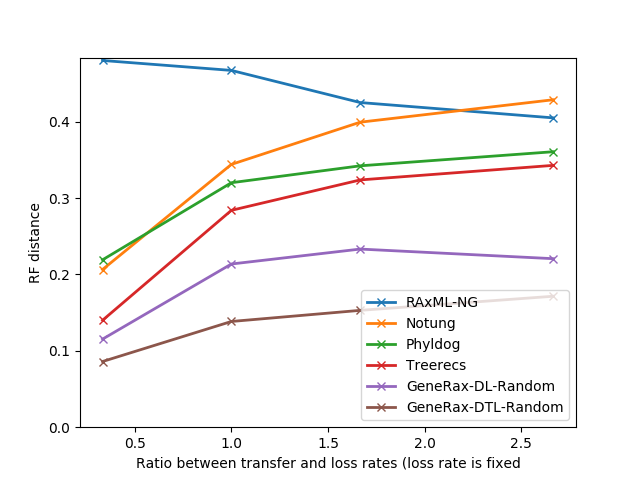
\includegraphics[scale=0.5]{transfers_dtl.png}
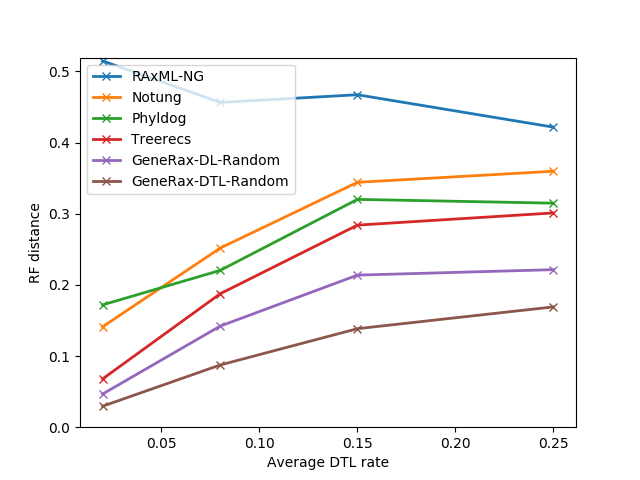
\includegraphics[scale=0.5]{dtl_rates_multiplier_dtl.png}
\end{figure}


\end{document}
